% Document Preamble
\documentclass{beamer}
\usetheme{metropolis}
%\usepackage{color}
%\usepackage[british]{babel}


\title{NOVA Shields with Tungsten $^{222}$Rn Emanation Measurement}
\author[R. Glayzer]{Ryott Glayzer}
\institute[SDSMT]
{
    Lab Assistant\\
    SD Mines
}
\date[2023]{\today}
\logo{
\includegraphics[height=1cm]{SD_Mines.png}}

\begin{document}

\frame{\titlepage}

\begin{frame}{Sample Photos}
    \begin{figure}
        \centering
        
\includegraphics[width=0.6\textwidth]{gordon-ramsay.png}
        \caption{This is photo of Gordon Ramsay}
    \end{figure}
\end{frame}

\begin{frame}{Overview of Emanation}
    \begin{itemize}
        \item Sample was emanated twice throughout Fall 2021
        \begin{itemize}
            \item Total Hours Emanated: 981 H 
            \item Total Data Hours: 399 H
            \item Usable Data Hours: 246 H 
        \end{itemize}
        \item Assays indicate an emanation rate of 
        \textbf{5.16 $\pm$ 0.22 mBq}
        
    \end{itemize}
    
\end{frame}
\begin{frame}{Rate vs. Time, Run 679}
    \begin{figure}
        \begin{center}
            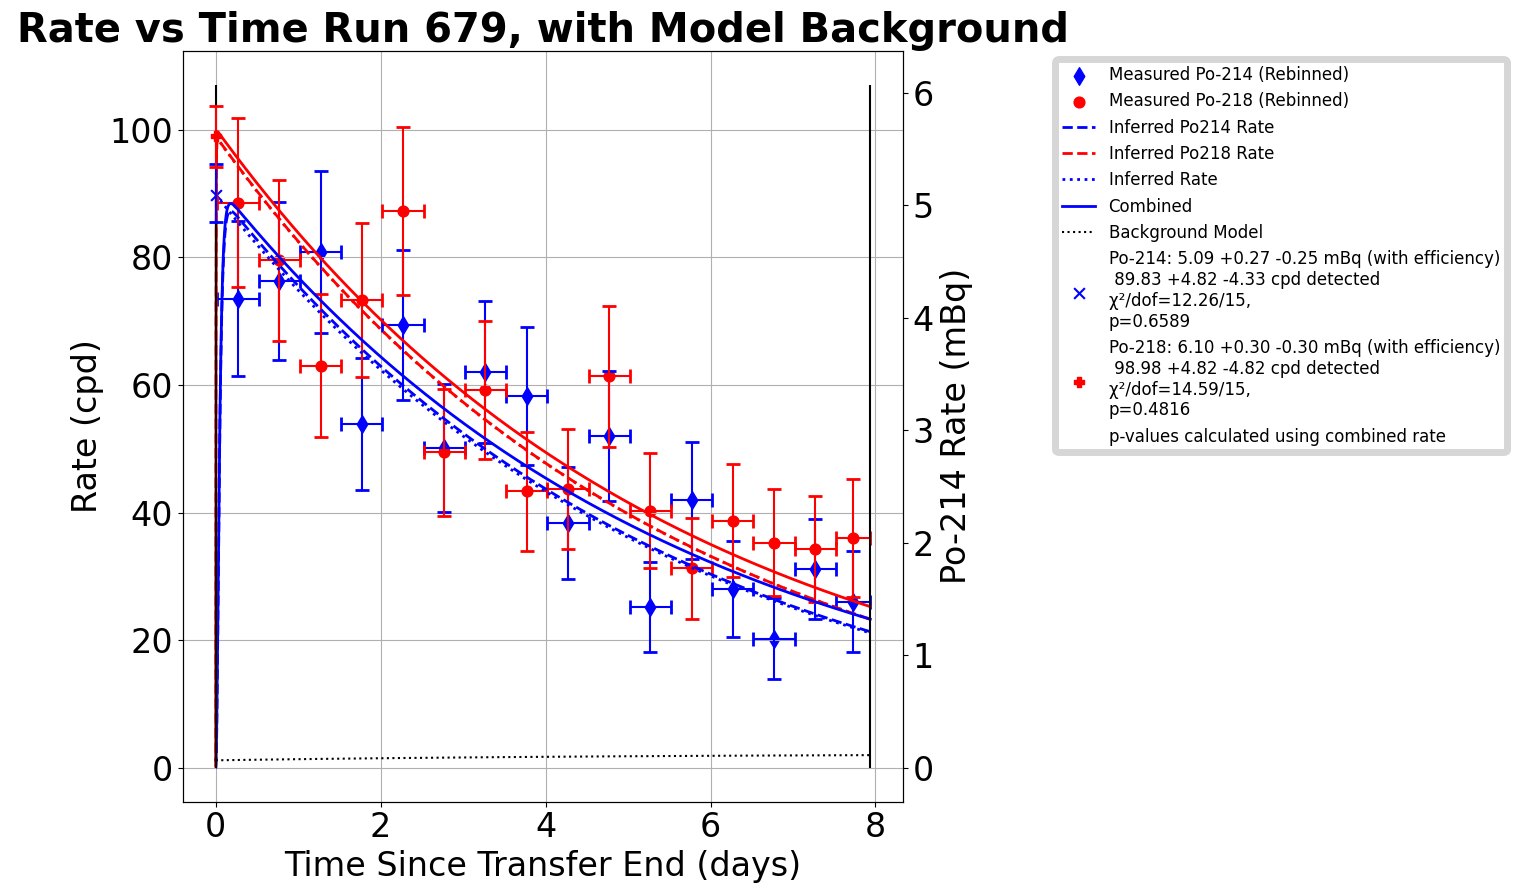
\includegraphics[width=0.9\textwidth]
            {Rate_vs_Time_Run_679,_with_Model_Background.png}
            \caption{$^{222}$Rn Emanation Rate: 
            \textbf{5.09 $\pm$ 0.26 mBq} (from $^{214}$Po Rate)}
        \end{center}
    \end{figure}  
\end{frame}

\begin{frame}{Rate vs. Time, Run 681}
    \begin{figure}
        \begin{center}
            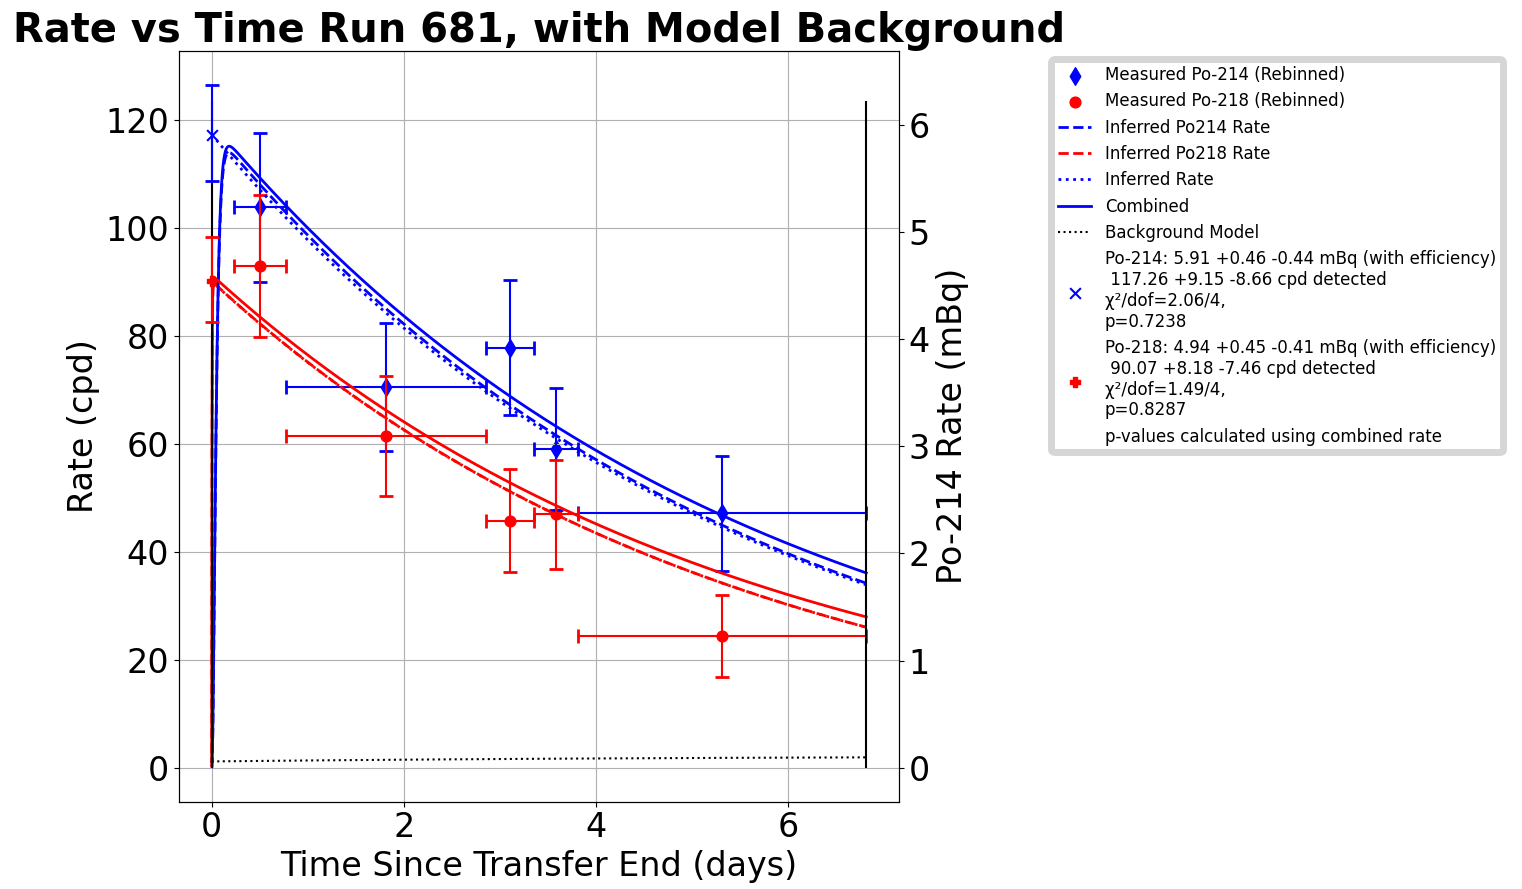
\includegraphics[width=0.9\textwidth]
            {Rate_vs_Time_Run_681,_with_Model_Background.png}
            \caption{$^{222}$Rn Emanation Rate: 
            \textbf{5.41 $\pm$ 0.48 mBq} (from $^{21x}$Po rates)}
        \end{center}
    \end{figure}    
\end{frame}

\begin{frame}{Summary of NOVA Shields with Tungsten Assay}
    
\end{frame}

\begin{frame}{Backup Slides}
    Backup Slides contain additional data and information that may be helpful
    to provide context if questions come up.
\end{frame}

\begin{frame}{Run 679 Data}
    The folowing slides contain data from Run 679, the first emanation of the 
    NOVA Shield with Tungsten.
\end{frame}
\begin{frame}{Run 679 Raw Data}
    \begin{figure}
        \begin{center}
            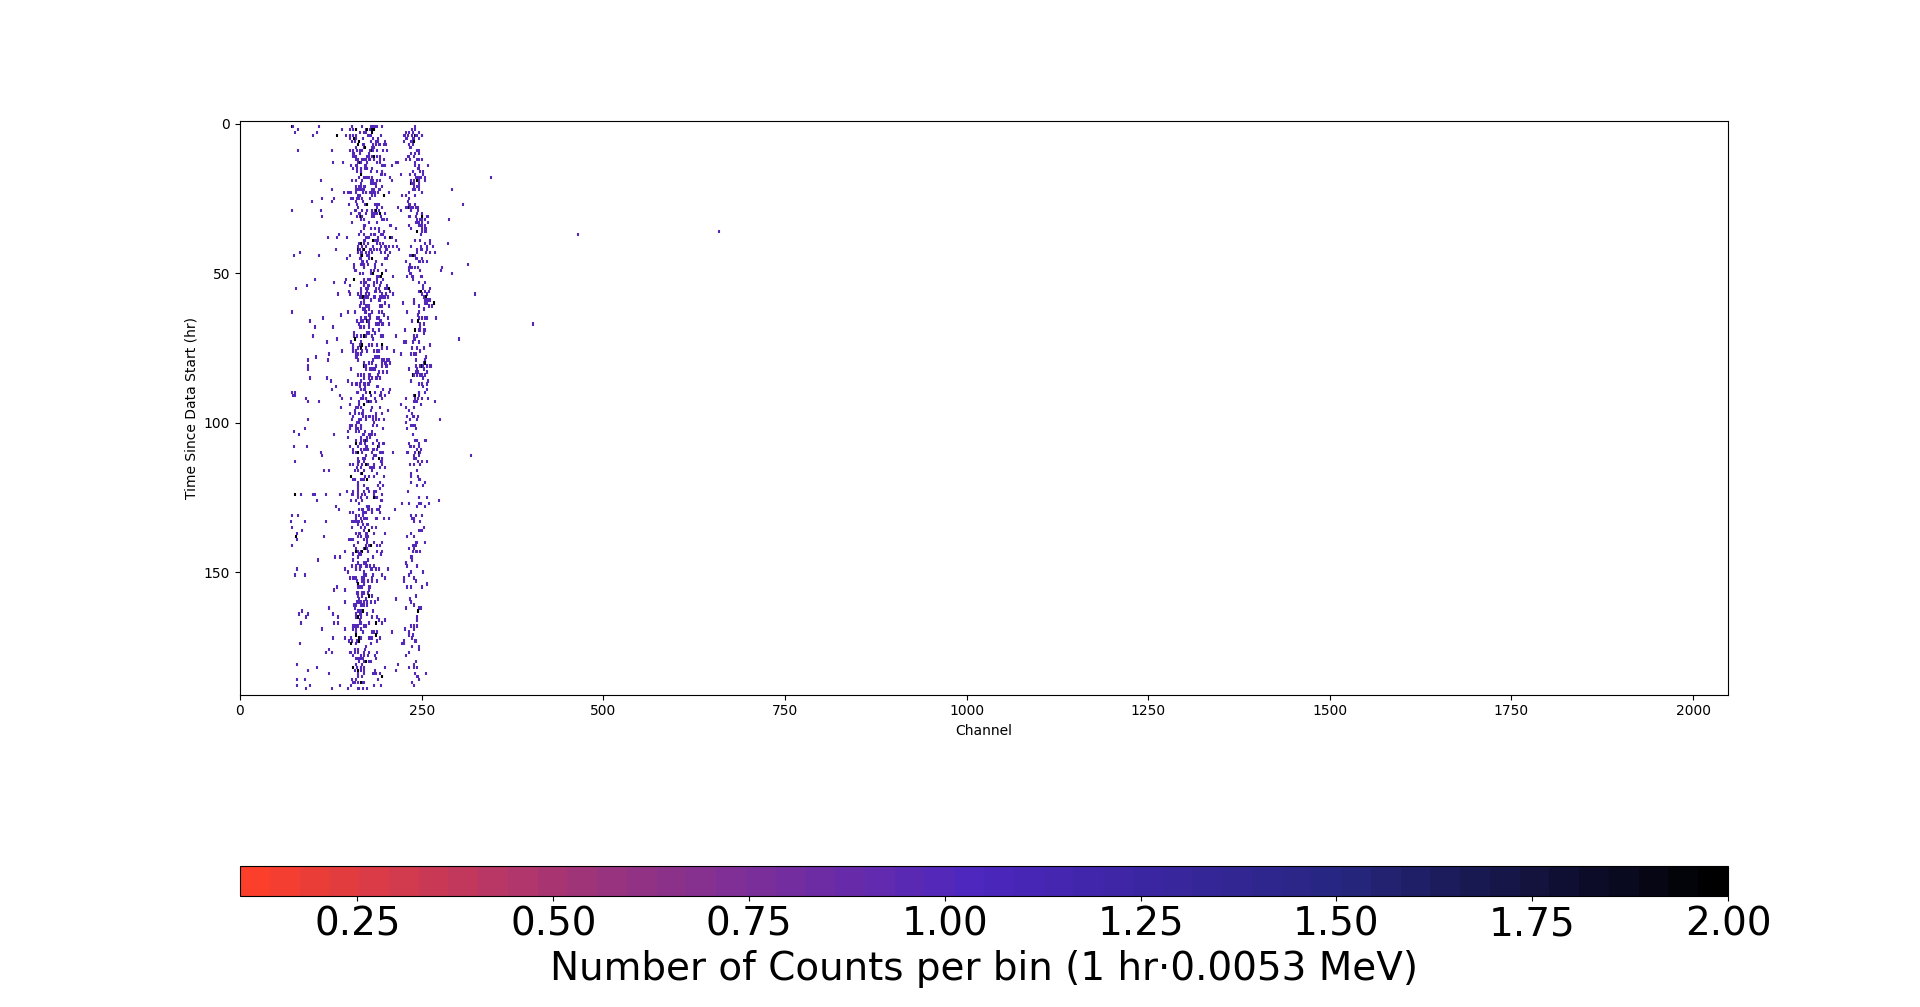
\includegraphics[width=\textwidth]{Run_679_Raw_Data.png}
        \end{center}
    \end{figure}
\end{frame}
\begin{frame}{Run 679 Gain-Corrected Data}
    \begin{figure}
        \begin{center}
            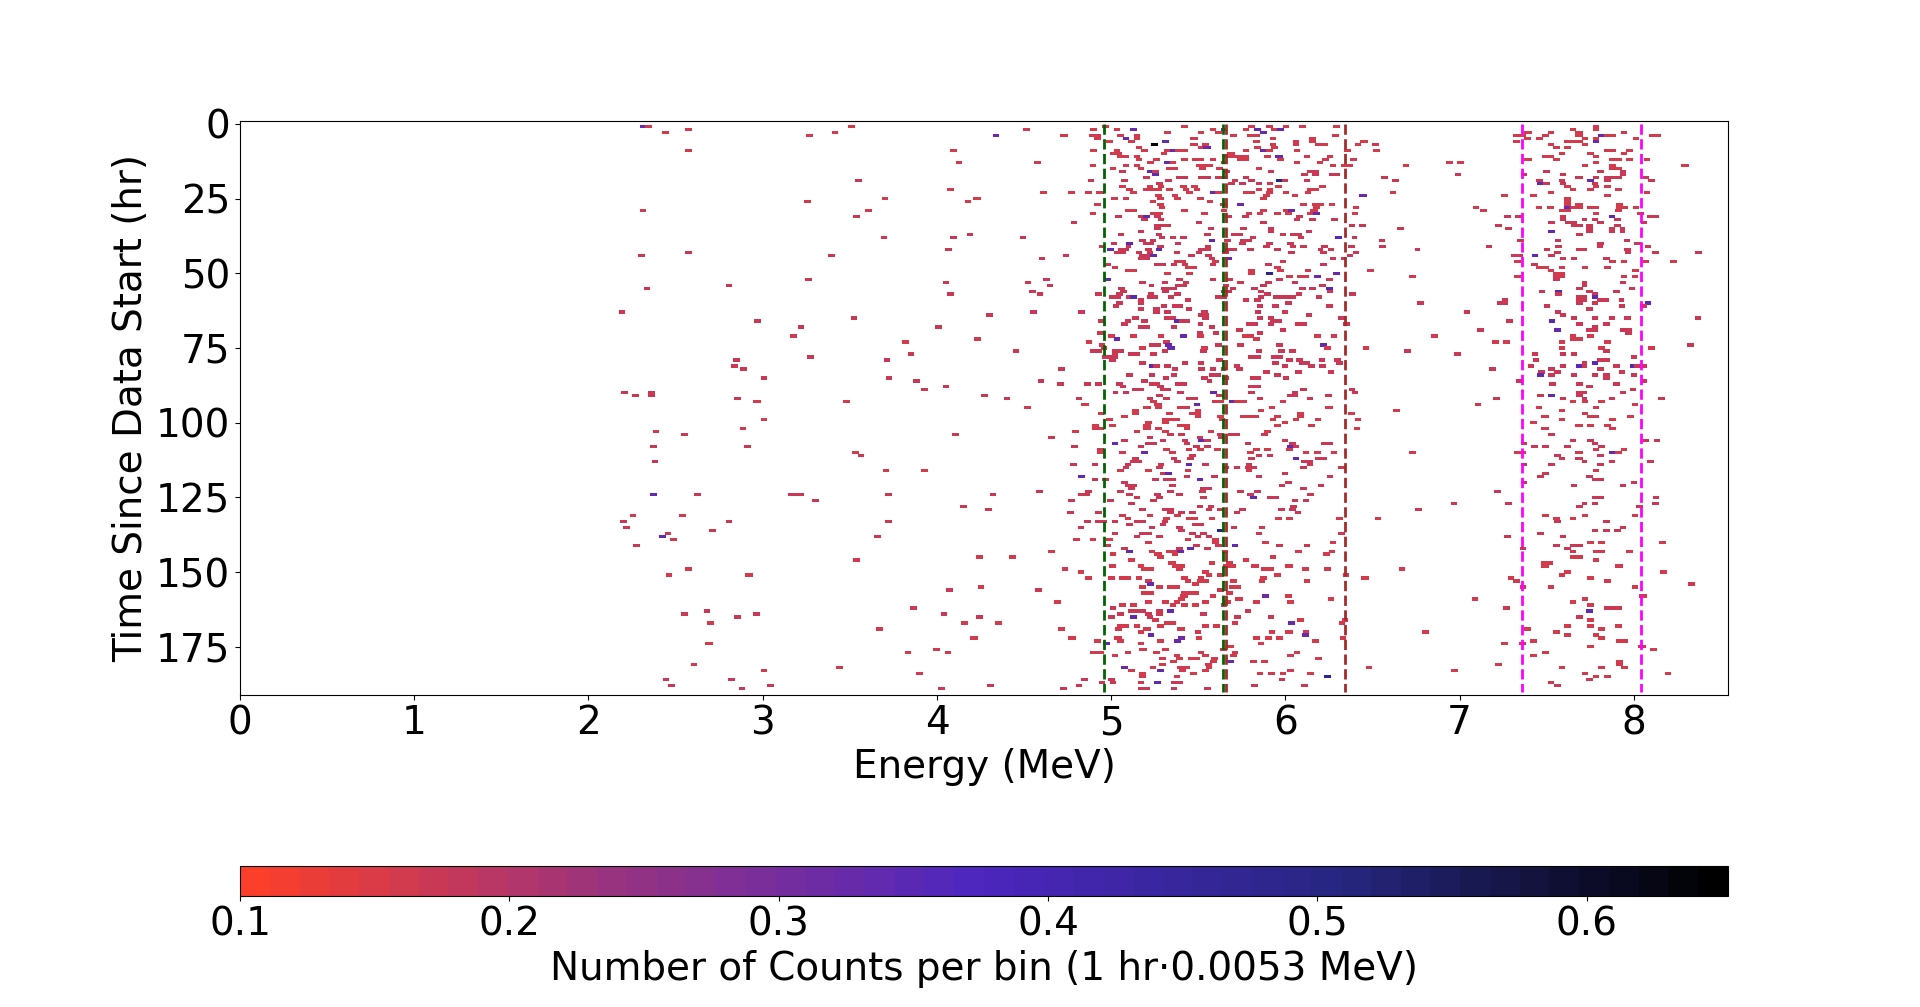
\includegraphics[width=\textwidth]{Run_679_Corrected_Data.png}
        \end{center}
    \end{figure}
\end{frame}



\begin{frame}{Run 681 Data}
    The folowing slides contain data from Run 681, the second emanation of the 
    NOVA Shield with Tungsten.
\end{frame}




\end{document}
